\documentclass[a4paper,10pt,onecolumn,oneside,titlepage]{article}

\usepackage[utf8]{inputenc}
\usepackage[spanish]{babel}
\usepackage{graphicx}
\usepackage[left=2cm,right=2cm,top=2cm]{geometry}
\usepackage{float}
\usepackage{rotating}
\usepackage{color}
\usepackage{xcolor}
\usepackage{listings}
\usepackage{caption}
%\usepackage{lscape}

\renewcommand{\baselinestretch}{1.5}
\addtolength{\parindent}{0pt}
\addtolength{\parskip}{\baselineskip}
\bibliographystyle{ieeetr}

\lstset{
% general command to set parameter(s)
basicstyle=\ttfamily, % print whole listing small
keywordstyle=\color{black}\bfseries\underbar, % underlined bold black keywords
identifierstyle=, % nothing happens
commentstyle=\color{white}, % white comments
stringstyle=\ttfamily, % typewriter type for strings
showstringspaces=false % no special string spaces
}

\title{Memoria Final - Sistemas Informáticos}
\author{Ignacio Robledo Rosell \\
				g990406}
\date{24 de Agosto de 2012}

\includeonly{
	introduccion,
	ficheroDWG,
	herramientas,
	plugin,
	alcance,
	desarrollos,
	pruebas,
	lineasFuturas,
	ap1-ejemploUso,
	ap2-ejemploSalida
}

\begin{document}

\maketitle

\tableofcontents

\section{Contexto.}

El contexto de este proyecto de SSII se engloba dentro del amplio mundo del \textit{Aprendizaje Automatico}
y del \textit{Reconocimiento de formas}.

\begin{itemize}

\item{Sistema A: Lectura e interpretaci�n del contenido de un fichero DWG.}
\item{Sistema B: Visualizaci�n y manipulado del contenido de un fichero DWG.}

\end{itemize}

Este proyecto se centra en el contexo del sistema A. El sistema B ser� desarrollado por otro alumno de la asignatura 
Sistemas Inform�ticos y ambos sistemas deber�n cooperar para cubrir las funcionalidades completas del proyecto.

Este trabajo dar� lugar tambi�n al proyecto fin de carrera de Ignacio Robledo Rosell. A lo largo del documento se 
describen algunas de las l�neas de trabajo futuras hac�a las que puede evolucionar el sistema con motivo del desarrollo
del proyecto fin de carrera.


\section{Formato de fichero DWG.}

Como ya se ha mencionado anteriormente, el formato de fichero DWG es un formato de fichero propietario, propiedad de la empresa Autodesk y no existe mucha información pública sobre el mismo. El fichero puede entenderse conceptualmente como una base de datos de objetos, muchos de ellos, con información geométrica asociada. Es una base de datos jerárquica donde todos los elementos tienen un identificador único. De una forma esquemática y simple, los objetos se agrupan del siguiente modo:

\begin{itemize}

\item{Un fichero DWG se compone de diferentes capas de información. Una capa es el objeto contenedor básico de elementos de AutoCad. Al menos siempre existe una capa, la denominada capa cero. El fichero puede contener cuantas capas desee el usuario.}

\item{Un fichero DWG se compone a su vez de diferentes bloques. Un bloque se forma a partir de uno o varios objetos combinados para crear un único objeto. Los objetos se distribuyen a través de las diferentes capas existentes en el fichero. Los bloques ayudan a volver a utilizar objetos en el mismo dibujo o en otros distintos. En todo fichero DWG existe al menos un bloque denominado \textit{Model Space} donde se guardan todos los objetos que crea el usuario si no indica que forman parte de un bloque diferente.}

\end{itemize}

Esa organización conceptual se traslada físicamente al fichero de forma que en el mismo se encuentran cuatro grandes secciones:

\begin{itemize}

\item{Sección de capas: contiene toda la información relativa a las capas existentes en el fichero DWG.}

\item{Sección de bloques: contiene la información de todos los bloques del fichero DWG, incluyendo la del bloque por defecto \textit{Model Space}.}

\item{Sección de otras tablas: contiene otra información necesaria para la gestión de un diseño, incluyendo información sobre los tipos de líneas disponibles, los estilos de texto disponibles, etc.}

\item{Sección de diccionarios: contiene diccionarios para dar cobertura a funcionalidades avanzadas del sistema AutoCad, como son diccionarios de materiales y de estilos visuales de presentación. Contiene también diccionarios personalizados por el usuario.}

\end{itemize}

A continuación se muestra un esquema de la organización de un fichero DWG:

\begin{figure}[h]
\begin{center}
\includegraphics[height=8cm]{imgs/dwgFile}
\caption{Esquema del contenido de un fichero DWG.}
\end{center}
\end{figure}

Cada elemento dentro de un fichero DWG contiene dos identificadores que permiten referenciar el objeto:

\begin{itemize}

\item{ObjetcId: Identificador único por instancia de AutoCAD. Un mismo fichero DWG abierto en dos instancias simultáneamente de AutoCAD tendrá dos ObjectID diferentes para cada una de las entidades, uno para cada instancia. Este identificador no es persistente y cada vez que se abre el fichero cambia.}

\item{HandleId: Identificador que puede no ser único por instancia de AutoCAD pero es persistente. Cada vez que se abre el fichero DWG, cada objeto tiene siempre el mismo valor para este identificador.}

\end{itemize}




\section{Herramientas para manipular ficheros DWG.}

Se ha establecido como requisito inicial que el proceso de extracción sea desarrollado con tecnología Java, dado que es una tecnología fiable y muy extendida y compatible con múltiples plataformas hardware / software. 

Con este requisito, se ha realizado una búsqueda de todas las herramientas disponibles en el mercado, libres / propietarias, gratuitas / con licencia, que permiten el manipulado, en modo lectura al menos, de un fichero con formato DWG. En esta búsqueda se han identificado las siguientes alternativas:

\begin{itemize}

\item{RealDWG \cite{RealDWG}: librería licenciada por la propia empresa AutoDesk para desarrollar software que pueda trabajar con ficheros DWG de una forma sencilla y documentada. Tiene un coste de licencia elevado, sobre los 5.000 dolares, y el proyecto en el que vaya a ser utilizada debe ser validado y autorizado por la propia empresa AutoDesk.}

\item{LibDWG \cite{LibDWG}: librería de código abierto desarrollada en lenguaje C que en teoría permite el acceso en modo lectura a un fichero DWG. El desarrollo de la misma se detuvo en Julio del 2009 y no existe una versión estable ni documentación ni ejemplos suficientes para su utilización.}

\item{LibreDWG \cite{LibreDWG}: librería de código abierto desarrollada por la comunidad GNU y basada en los desarrollos anteriores de LibDWG. El desarrollo de la misma esta en una fase alpha, no estable aún, y no existe una API correctamente documentada para trabajar con la misma. También esta desarrollada en lenguaje C.}

\item{DWGDirect \cite{OpenDWG}: librería desarrollada por la <<Open Design Alliance>>. Esta librería solo esta accesible para socios de la organización.}

\end{itemize}

Las conclusiones de la búsqueda no son muy satisfactorias. No parece existir una alternativa real y consolidada más alla de licenciar a la propia compañía AutoDesk el kit de desarrollo RealDWG. Ninguna alternativa de las mencionadas anteriormente contempla Java como tecnología a utilizar.

La <<Open Design Alliance>> no publica su librería para trabajar con ficheros DWG fuera de sus socios y miembros pero sin embargo publica y libera periódicamente una especificación del formato interno del fichero DWG. Esta especificación se obtiene a través de mecanismos de ingeniería inversa. La última especificación disponible aparentemente da soporte a los formatos del fichero DWG desde la versión 13 de AutoCAD hasta las versiones 2010-2012. 

Analizando la situación se opta por desarrollar un interprete nativo en Java, siguiendo las especificaciones publicadas por la <<Open Design Alliance>>. Tras unos dias de intenso desarrollo, empieza a ser una realidad que esta elección no es la mejor, dado que las especificaciones son complejas, incompletas y va a requerir mucho más tiempo del planificado, desarrollar una libreria Java capaz de interprentar minimamente un fichero con formato DWG, superando con creces el alcance de un proyecto de SSII.

Llegado este punto, se realiza una nueva valoración de las alternativas ya expuestas anteriormente. Se valorá la posibilidad de trabajar con la librería LibreDWG, aunque no sea bajo la tecnología Java, dado que lo importante para el proyecto es ser capaces de extraer la información del fichero DWG y ponerla a disposición de otros sistemas informáticos en un formato legible y sencillo de tratar. La tecnología debe ser un medio y no un fin en si mismo. Una vez tomada la decisión de abandonar Java como lenguaje de programación, se realiza una nueva búsqueda y se encuentra una posible alternativa no localizada en la primera selección de herramientas. 

Se localiza la librería ObjectARX \cite{ObjectARX}, librería proporcionada por la propía compañía AutoDesk para el desarrollo de plugins para su colección de herramientas, incluyendo el propio AutoCAD. Permite el desarrollo de los plugins en lenguaje C++ y en lenguajes disponibles en la plataforma .NET (C\# y VB .NET). Y lo mas importante, proporciona una API bien documentada y estable para el acceso y manipulado de ficheros DWG.

Dado que el formato DWG y el AutoCAD son un estandar de facto en el sector de las infraestructuras aeronáuticas, se presupone que los usuarios finales del proceso extractor dispondran del propio software AutoCAD. Por ello, finalmente, se decide desarrollar el proceso extractor como un plugin que trabajará directamente en la propia herramienta AutoCAD y será desarrollado con tecnología .NET, en concreto C\#. 

Estos nuevos requerimientos difieren técnicamente de los inicialmente propuestos pero dada la escasa viabilidad del planteamiento inicial se ha procedido a buscar una solución que permita obtener resultados funcionales completamente funcionales y adaptar los requisitos técnicos a la propuesta más viable.


\section{¿Cómo trabaja un plugin para AutoCAD?.}

La propia empresa AutoDesk proporciona los materiales necesarios para que sus usuarios desarrollen sus propios plugins y puedan personalizar y extender las funcionalidades de sus herramientas. Con un enfoque comercial muy interesante, si un usuario consigue sentirse comodo y personalizar una herramienta de forma sencilla, conseguiras retenerle de una forma simple y conseguir que continue trabajando con tu herramienta de forma sistemática en el tiempo.

En concreto, la propia empresa AutoDesk justifica su elección de la plataforma .NET para dotar de estas capacidades al usuario de sus herramientas:

\begin{itemize}

\item{.NET es una herramienta de desarrollo estandarizada en el mercado y soportada por una gran compañía como es Microsoft.}

\item{.NET proporciona una gran colección de librerias y métodos listos para ser usados dentro del entorno de ejecución de .NET}

\item{Rápida curva de aprendizaje, en poco tiempo estas completando tus primeros desarrollos.}

\item{Buen soporte de tipos: tipos básicos y tipos más complejos, como colecciones.}

\item{Buen entorno de desarrollo, con sus versiones gratis y profesionales.}

\end{itemize}

La tecnología .NET es usada en la mayoría de los productos de la compañía AutoDesk. La mayoría de los productos exponen sus funcionalidades a través de una API bien documentada en tecnología .NET.

El proceso de desarrollo es bastante sencillo. Tan solo hay que seguir los siguientes pasos:

\begin{itemize}

\item{Referenciar en el proyecto las dos librerias a través de las que el producto AutoCAD expone sus servicios al entorno .NET: AcDbMgd.dll y AcMgd.dll.}

\item{Desarrollar el código del plugin con el lenguaje escogido y las librerias estandar proporcionadas por el entorno .NET, la API proporcionada por AutoCAD y cualquier API de terceros que se pueda necesitar.}

\item{No es necesario extender ninguna clase específica para crear el plugin. Cualquier clase pública es válida y tan sólo debe anotarse el método que vaya a contener toda la lógica del mismo con la anotación <<CommandMethod>>. Esta anotación permite a AutoCAD indentificar los nuevos comandos implementados en el plugin y hacerlos accesibles al usuario final.}

\item{Compilar el proyecto y generar un ensamblado final con todos los componentes, archivo .DLL}

\item{Cargar el ensamblado desde el entorno .NET a través del comando NETLOAD.}

\item{Invocar el comando o comandos definidos en el plugin.}

\end{itemize}

\begin{figure}[H]
\begin{center}
\includegraphics[height=8cm]{imgs/plugin}
\caption{Esquema del proceso de desarrollo de un plugin para AutoCAD \cite{AutoCAD-NET-API}.}
\end{center}
\end{figure}

\section{Definición del alcance. Requisitos funcionales.}

Dada la complejidad de los ficheros DWG, que contienen gran cantidad de información diferente, se ha definido el siguiente alcance para el proyecto de Sistemas Informáticos:


\begin{itemize}

\item{Req 1: Abrir y manipular un fichero en formato DWG en modo lectura.}
\item{Req 2: Identificar las capas existentes dentro del fichero.}
\item{Req 3: Identificar los objetos de tipo punto existentes dentro del fichero.}
\item{Req 4: Identificar los objetos de tipo línea existentes dentro del fichero.}
\item{Req 5: Identificar los objetos de tipo polilínea existentes dentro del fichero.}
\item{Req 6: Identificar los objetos de tipo arco existentes dentro del fichero.}
\item{Req 7: Identificar los siguientes atributos para cada uno de los elementos anteriores: color, grosor de la línea, capa a la que pertenecen}.
\item{Req 8: Almacenar la información obtenida de cada uno de los elementos en una estructura de objetos en memoria que en futuros desarrollos pueda ser utilizada}.
\item{Req 9: Exportar a un fichero de intercambio el contenido de esa estructura de objetos en memoria para ser utilizado por otros procesos, y más en concreto, por el proceso visualizador que se esta desarrollando en otro proyecto de SSII.}
\item{Req 9: Permitir al usuario indicar la ruta donde quiere guardar el fichero de intercambio}.
\item{Req 10: Permitir al usuario seleccionar que capas deben ser procesadas en busca de los objetos y cuales deben ser omitidas del proceso de búsqueda.}.
\item{Req 11: Para los objetos de tipo polilínea y de tipo arco obtener un conjunto de objetos de tipo línea alternativos que permitan dibujar una aproximación gráfica de la polilínea o del arco en un entorno visual en el que sólo se puedan dibujar líneas.}.

\end{itemize}

\section{Desarrollo.}
El Sistema Informático desarrollado se compone de 3 módulos / elementos que de forma conjunta proveen de la funcionalidad necesaria a AutoCAD para exportar los elementos del fichero DWG a un fichero en un formato XML. Estos módulos se apoyan en los siguientes componentes que el propio AutoCAD expone a disposición de los desarrolladores:

\begin{itemize}

\item{AutoDesk.AutoCAD.Runtime: este módulo inicializa los servicios de la aplicación cliente y las factorias que producen los diferentes objetos para ser utilizados dentro del entorno .NET.}

\item{AutoDesk.AutoCAD.ApplicationServices: este módulo permite la interacción con la aplicación AutoCAD. Provee acceso a los módulos adicionales como el editor, el gestor de documentos, ventana principal, etc.}

\item{AutoDesk.AutoCAD.DatabaseServices: esto módulo permite la interacción con el fichero de dibujo AutoCAD (DWG). Permite el acceso al header del mismo, a las tablas de símbolos, a las tablas de registros de entidades y a los diferentes objetos que componen el dibujo.}

\item{AutoDesk.AutoCAD.Geometry: esto modulo permite la interacción con el servicio de geometría de AutoCAD que se encarga de la gestión de las referencias espaciales.}

\item{AutoDesk.AutoCAD.EditorInput: esto modulo permite la interacción con el editor a través del cual se realiza la interacción con el usuario en ambos sentidos.}

\end{itemize}

Los 3 módulos / elementos desarrollados son:

\begin{itemize}

\item{dwgElementos: este módulo contiene las clases necesarias para representar y almacenar en memoria la información contenida en un fichero con formato DWG. En concreto esta formado por las clases:}

\begin{itemize}

\item{dwgPunto}
\item{dwgLinea}
\item{dwgArco}
\item{dwgPolylinea}
\item{dwgCapa}
\item{dwgFile}

\end{itemize}

\item{AutoDesk.AutoCAD.ApplicationServices: este módulo permite la interacción con la aplicación AutoCAD. Provee acceso a los módulos adicionales como el editor, el gestor de documentos, ventana principal, etc.}

\item{AutoDesk.AutoCAD.DatabaseServices: esto módulo permite la interacción con el fichero de dibujo AutoCAD (DWG). Permite el acceso al header del mismo, a las tablas de símbolos, a las tablas de registros de entidades y a los diferentes objetos que componen el dibujo.}

\item{AutoDesk.AutoCAD.Geometry: esto modulo permite la interacción con el servicio de geometría de AutoCAD que se encarga de la gestión de las referencias espaciales.}

\item{AutoDesk.AutoCAD.EditorInput: esto modulo permite la interacción con el editor a través del cual se realiza la interacción con el usuario en ambos sentidos.}

\end{itemize}

\section{Pruebas.}

Para verificar el correcto funcionamiento del plugin se realizan diferentes pruebas de exportación de diferentes grados de dificultad. Las primeras pruebas sencillas consisten en la exportación del contenido de ficheros DWG con contenidos básicos:

\begin{itemize}

\item{Fichero con una o varias líneas.}
\item{Fichero con una polilínea}
\item{Fichero con varias polilíneas}
\item{Fichero con un arco}
\item{Fichero con varios arcos}
\item{Fichero combinando todos los elementos anteriores en una sola capa.}
\item{Fichero combinando todos los elementos anteriores en varias capas.}

\end{itemize}

Los resultados de estas pruebas son satisfactorios.

En una segunda fase se obtiene a través del distribuidor de AutoCAD varios ejemplos de ficheros de complejidad media con combinaciones de capas y objetos más complejos.

Los resultados de estas pruebas también son satisfactorios. 

Superados los dos primeros conjuntos de pruebas, se procede a probar con uno de los ficheros originales, utilizados en \cite{Miguel-Munoz}, que se ha establecido como la prueba de validación y verificación del correcto funcionamiento del proceso de exportación. 

Los resultados son totalmente satisfactorios. A continuación puede verse una captura de pantalla del módulo de visualización realizado por otro alumno que se alimenta del fichero XML generado por el plugin. También se muestra para poder validar el resultado final, el fichero original DWG mostrado por la aplicación AutoCAD.

\begin{figure}[H]
\begin{center}
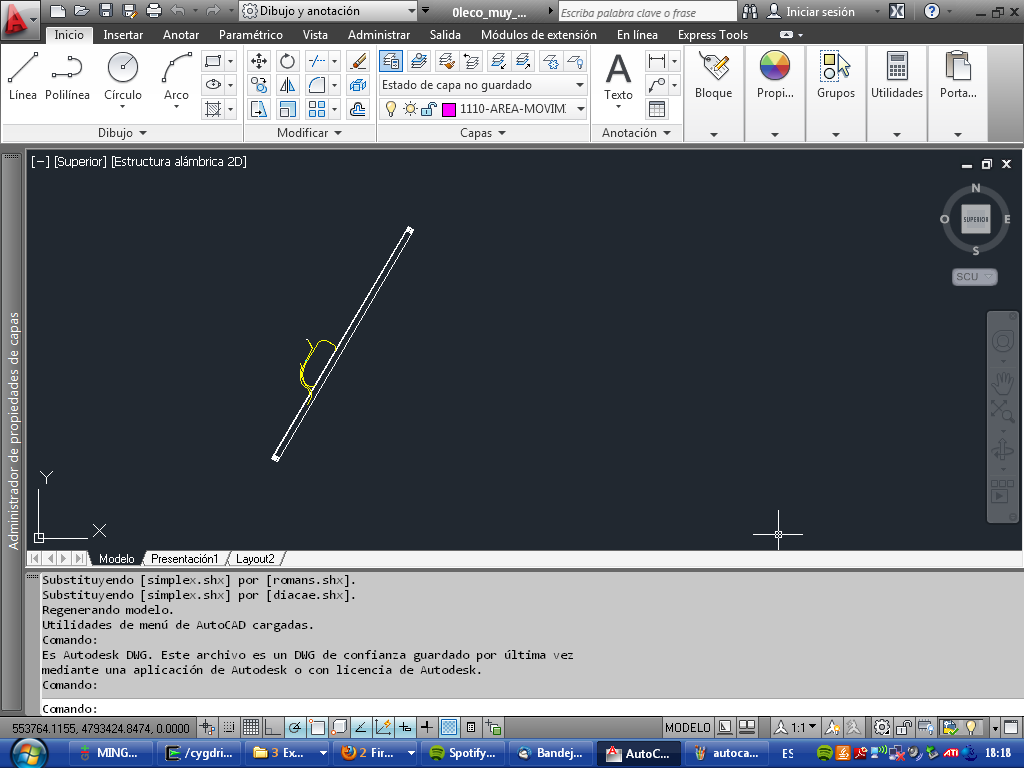
\includegraphics[width=0.8\textwidth]{imgs/autocad2}
\caption{Aplicación AutoCAD mostrando fichero DWG.}
\end{center}
\end{figure}

\begin{figure}[H]
\begin{center}
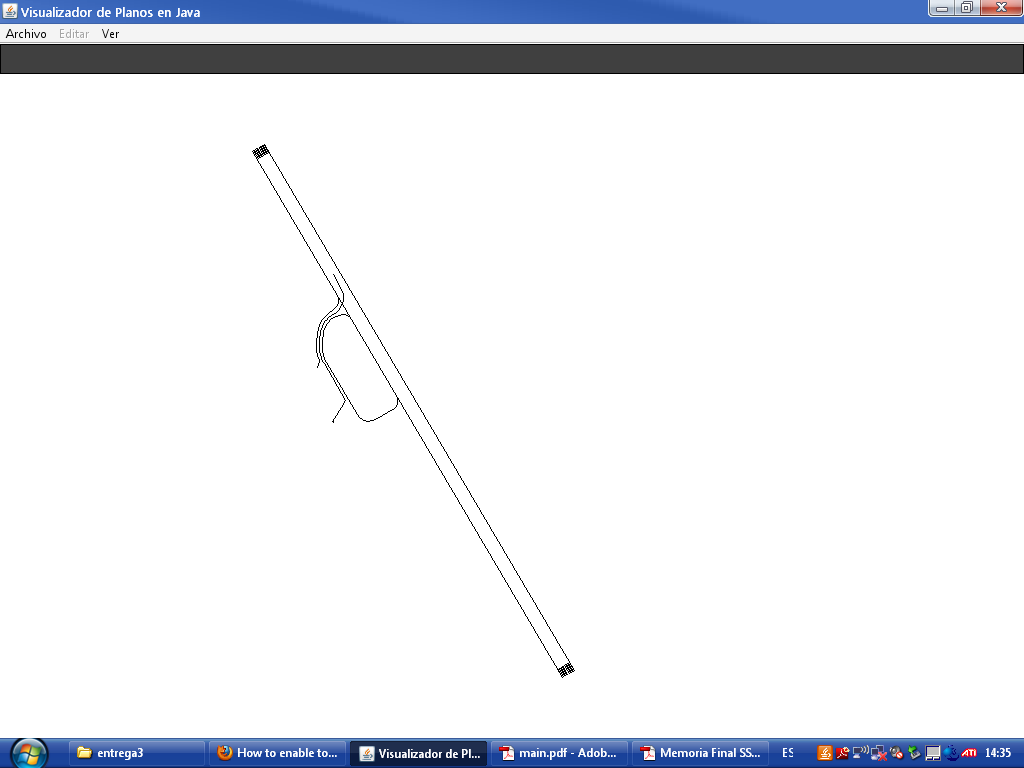
\includegraphics[width=0.8\textwidth]{imgs/ejemplo_salida}
\caption{Módulo visualizador mostrando el contenido del fichero DWG a partir del XML de intercambio.}
\end{center}
\end{figure}

En una última fase de pruebas se quiere verificar la consistencia del proceso ante ficheros muy complejos. Se obtiene a través del distribuidor de AutoCAD dos ejemplos de ficheros del diseño de una planta de un edificio nuevo con miles de objetos de distintos tipos en su interior y gran cantidad de capas. 

En esta última fase los resultados son también satisfactorios completándose correctamente la fase de exportación en un tiempo bastante reducido.

Por tanto, tras todas estas pruebas, puede considerarse verificado el correcto funcionamiento del plugin y la consistencia del mismo.
\section{Líneas futuras de trabajo.}

Una vez completado el alcance definido para el proyecto de Sistemas Informáticos se abre la cuestión de cuales pueden ser las posibles líneas futuras de trabajo para este sistema. Llegados a este punto y con el aprendizaje obtenido durante el desarrollo del mismo, se hace necesario replantear el proyecto inicial de construir un sistema independiente que limpie y optimice los diseños de nuevas infraestructuras para ser utilizadas en los simuladores de tiempo avanzado. 

¿Es realmente necesario que el sistema sea independiente? Quizás sea más efectivo proporcionar una serie de plugins para la herramienta AutoCad que permitan cubrir todas las etapas del sistema:

\begin{itemize}

\item{Etapa 1. Identificar y obtener la información geométrica de los diferentes elementos contenidos en un fichero DWG.}
\item{Etapa 2. Aplicar técnicas de aprendizaje automático y reconocimiento de formas para identificar las diferentes estructuras complejas contenidas en el fichero y adaptarlas y formatearlas a los requisitos de los diferentes simuladores.}
\item{Etapa 3: Escritura de esas nuevas estructuras adaptadas en un fichero con un formato reconocido por los distintos simuladores.}

\end{itemize}

Las líneas futuras de trabajo para la etapa 1 es continuar reconociendo tipos de objetos y estructuras adicionales y realizar baterías de pruebas más extensas con materiales reales.

Para las etapas 2 y 3 se hace necesario desarrollar algún tipo de prototipo que muestre la viabilidad de este planteamiento para posteriormente, si se dan las condiciones favorables, desarrollar los plugins que permitan completar el funcionamiento global del sistema.
\section{Apendice 1. Ejemplo de utilización del plugin SERIALIZARDWG.}

\begin{figure}[h]
\begin{center}
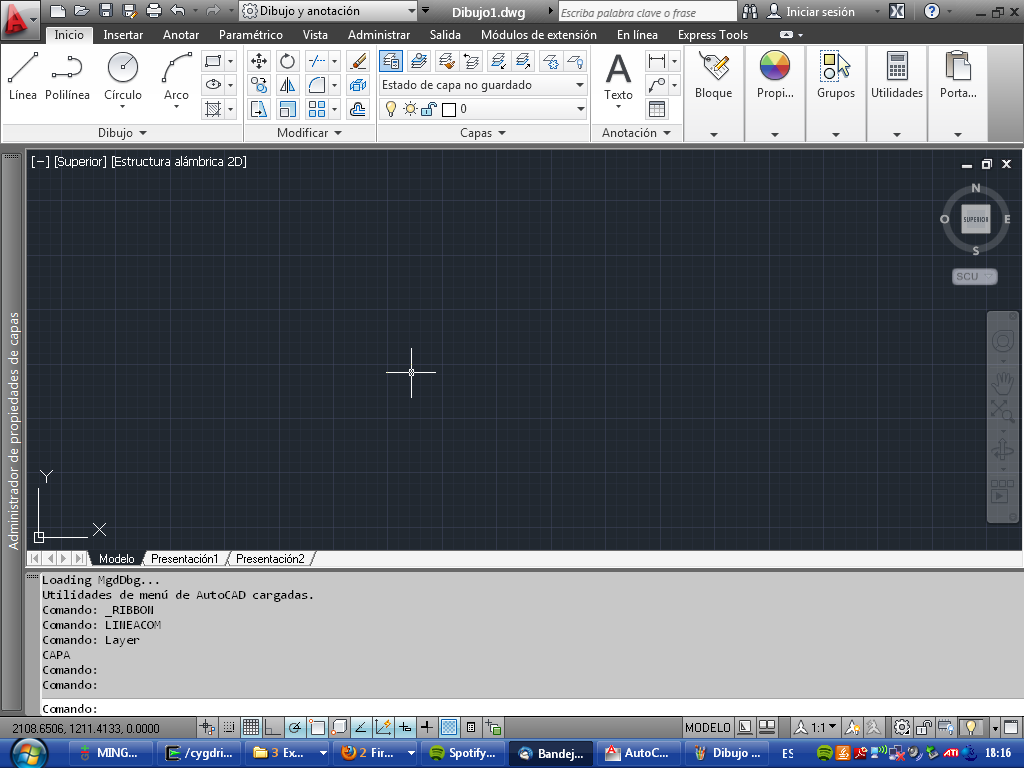
\includegraphics[width=\textwidth]{imgs/autocad0}
\caption{Aplicación AutoCAD.}
\end{center}
\end{figure}


\begin{figure}[h]
\begin{center}
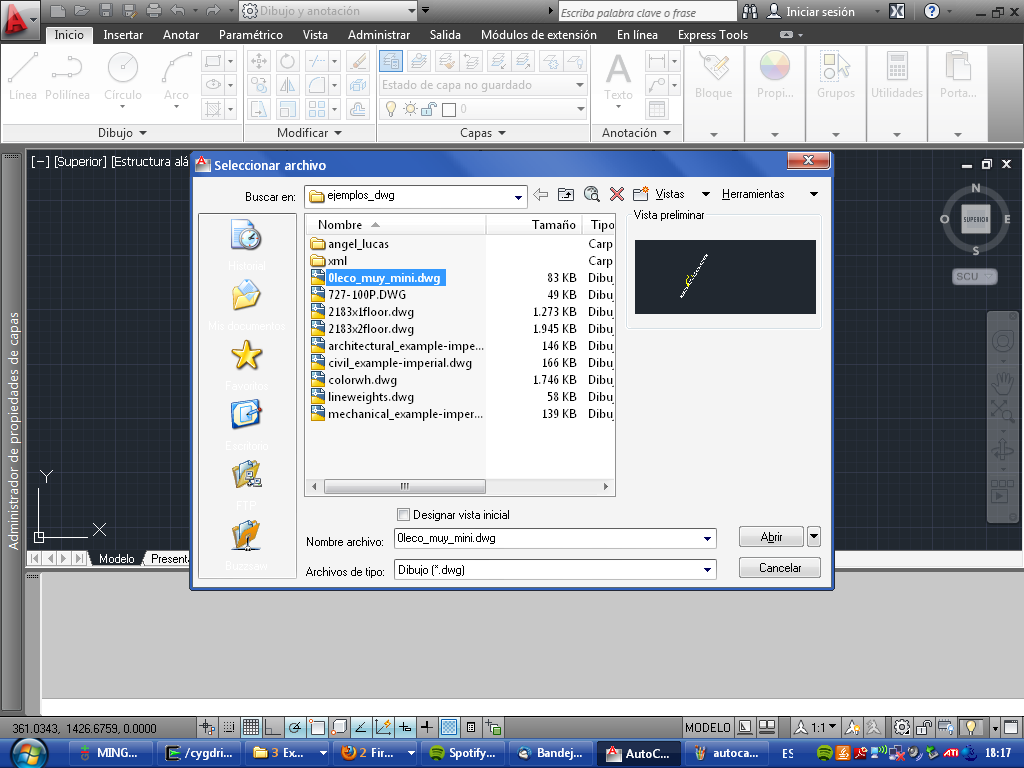
\includegraphics[width=\textwidth]{imgs/autocad1}
\caption{Aplicación AutoCAD abriendo fichero DWG.}
\end{center}
\end{figure}

\begin{figure}[h]
\begin{center}
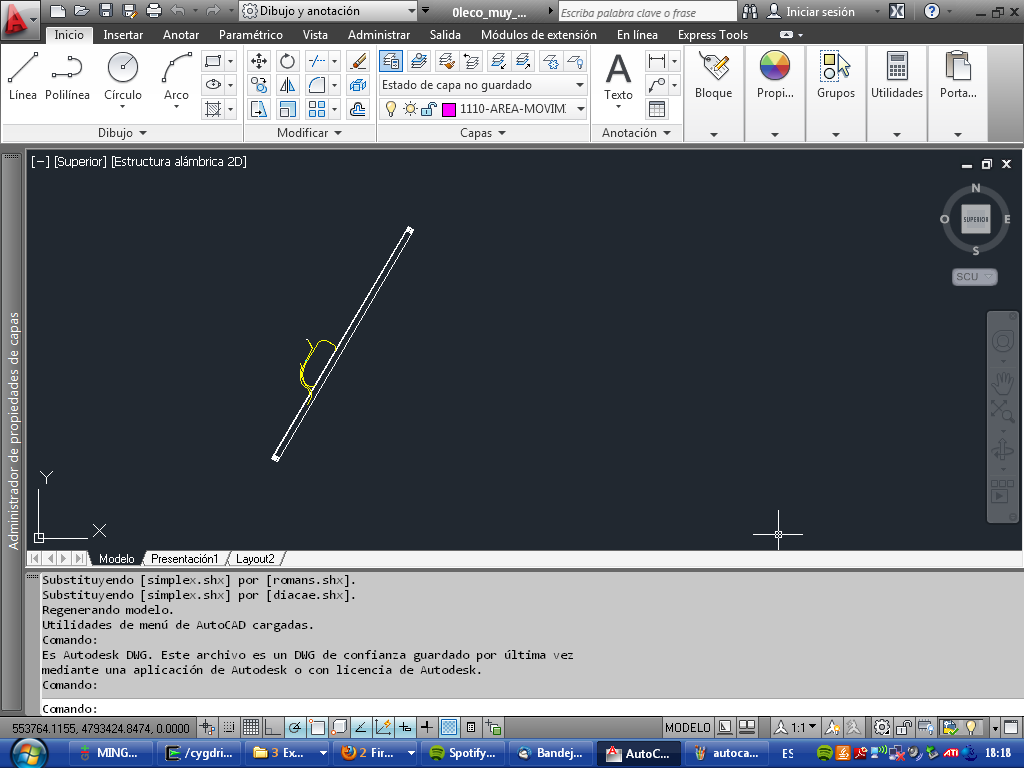
\includegraphics[width=\textwidth]{imgs/autocad2}
\caption{Aplicación AutoCAD mostrando fichero DWG.}
\end{center}
\end{figure}

\begin{figure}[h]
\begin{center}
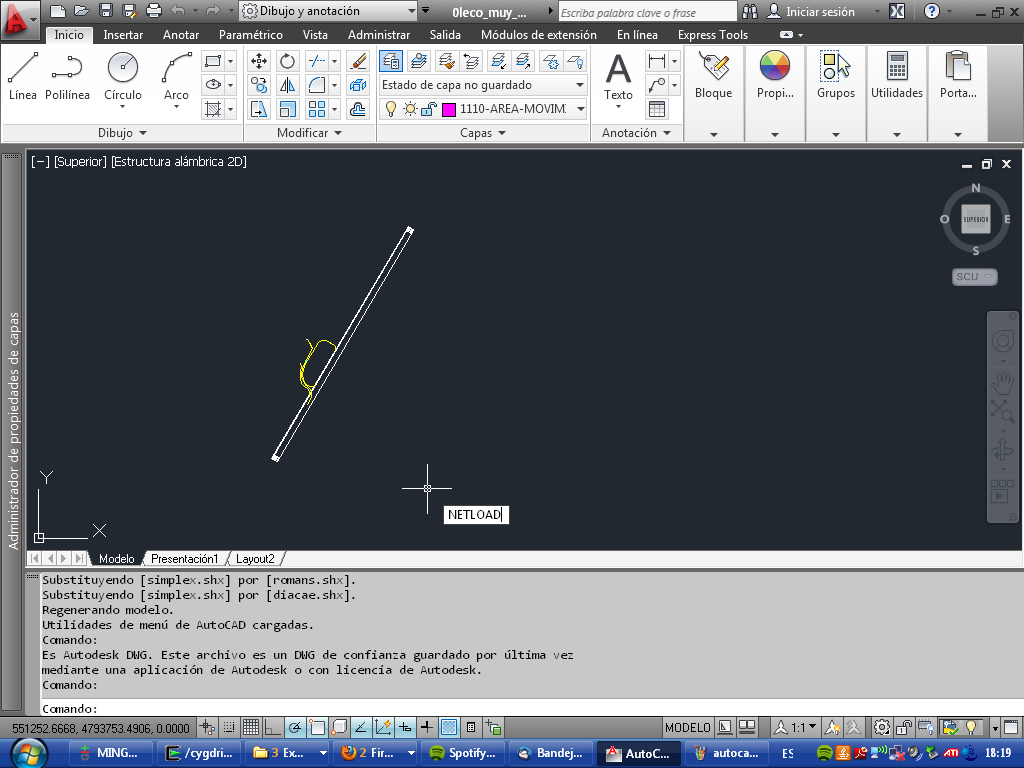
\includegraphics[width=\textwidth]{imgs/autocad3}
\caption{Invocacion del comando NETLOAD para cargar el plugin.}
\end{center}
\end{figure}

\begin{figure}[h]
\begin{center}
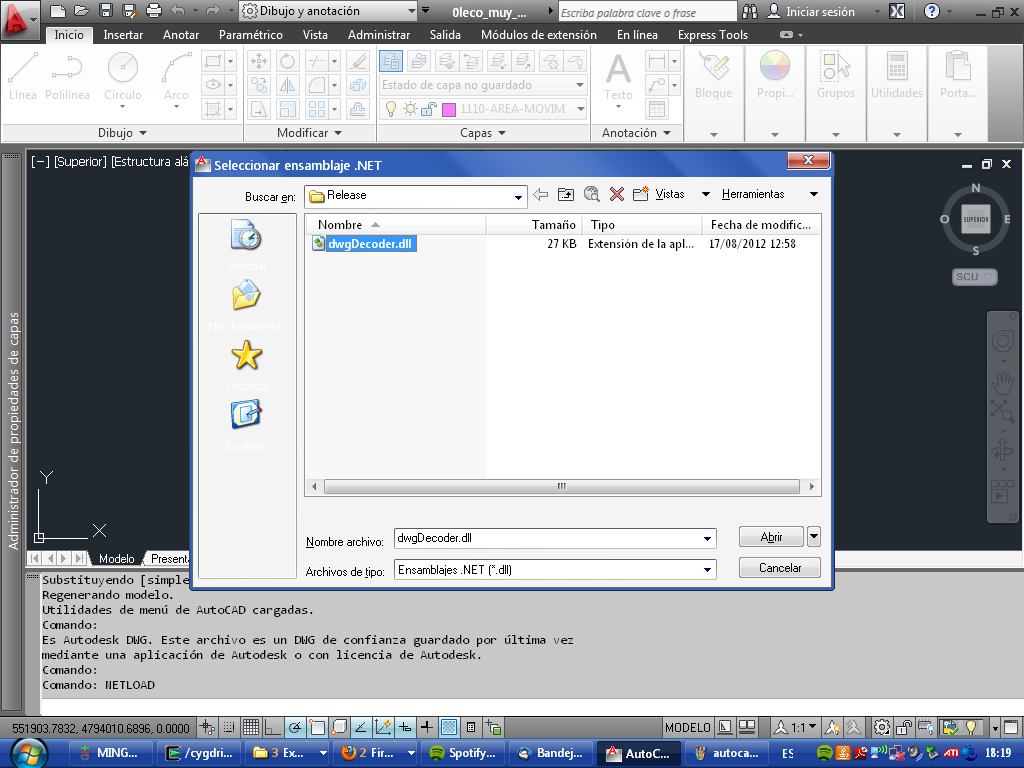
\includegraphics[width=\textwidth]{imgs/autocad4}
\caption{Selección del fichero DLL que cotiene el plugin.}
\end{center}
\end{figure}

\begin{figure}[h]
\begin{center}
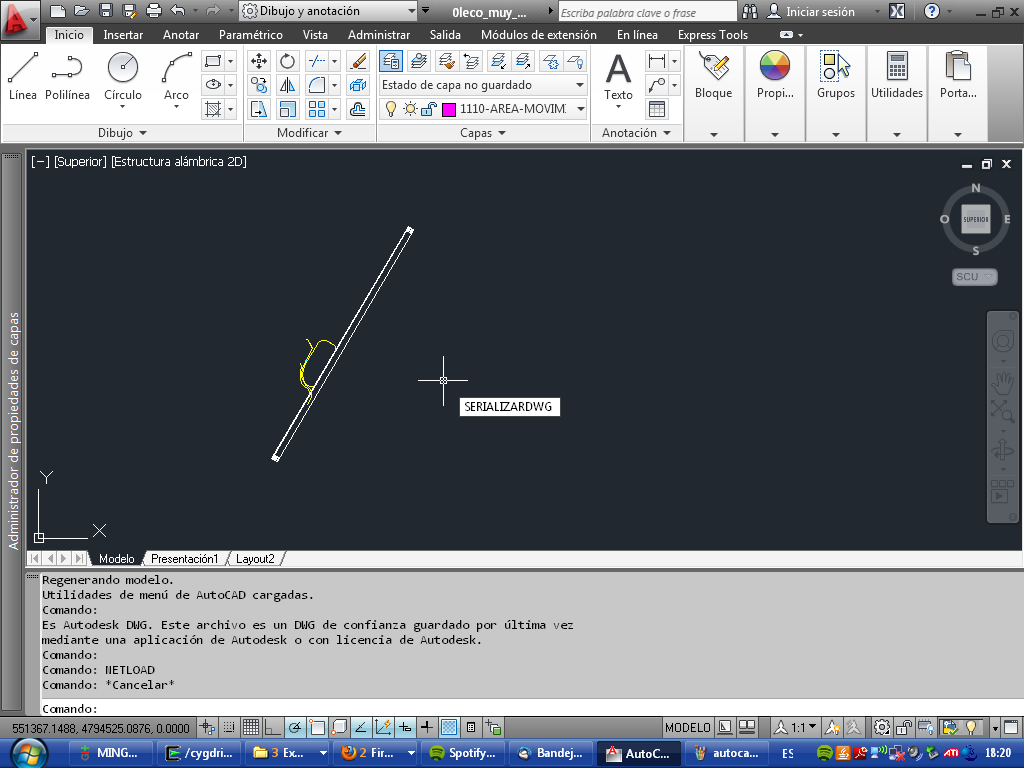
\includegraphics[width=\textwidth]{imgs/autocad5}
\caption{Invocación del comando SERIALIZARDWG implementado en el plugin.}
\end{center}
\end{figure}

\begin{figure}[h]
\begin{center}
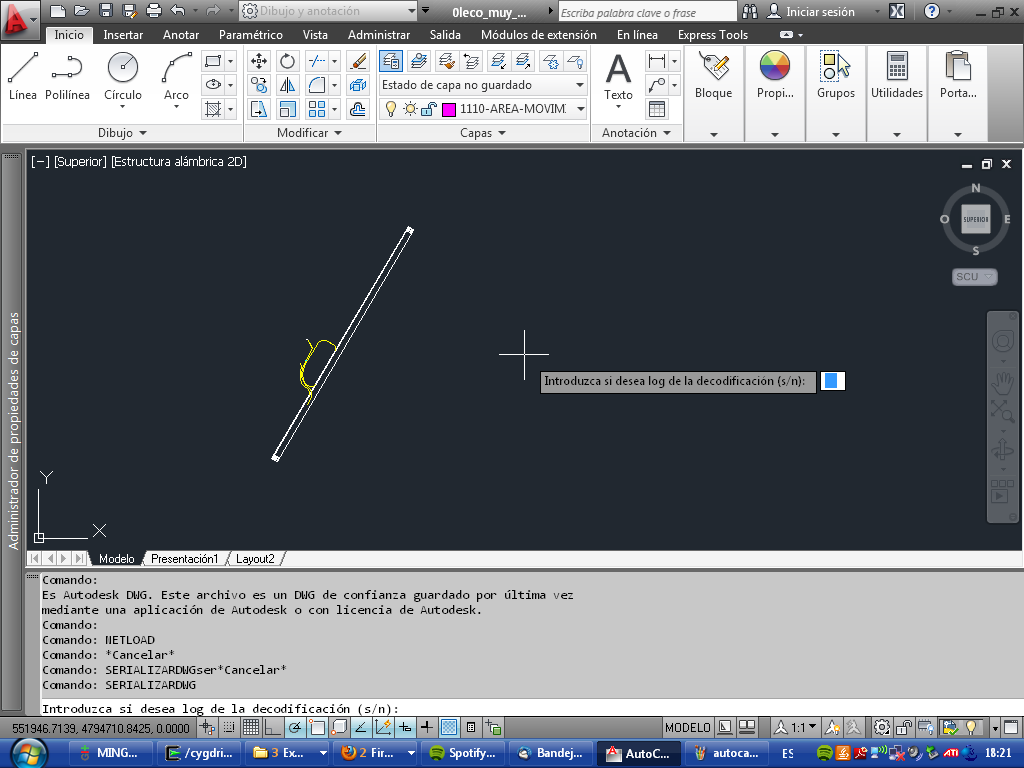
\includegraphics[width=\textwidth]{imgs/autocad6}
\caption{Usuario configurando si desea log del proceso de extracción.}
\end{center}
\end{figure}

\begin{figure}[h]
\begin{center}
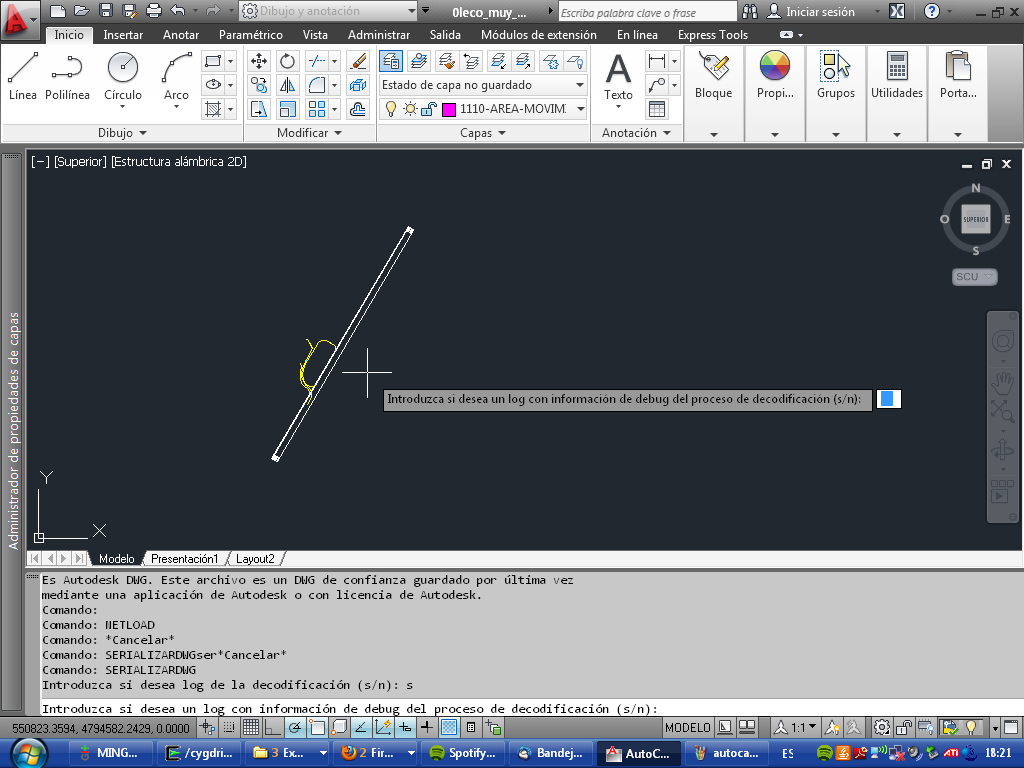
\includegraphics[width=\textwidth]{imgs/autocad7}
\caption{Usuario configurando si desea incorporar información de debug al log del proceso de extracción.}
\end{center}
\end{figure}

\begin{figure}[h]
\begin{center}
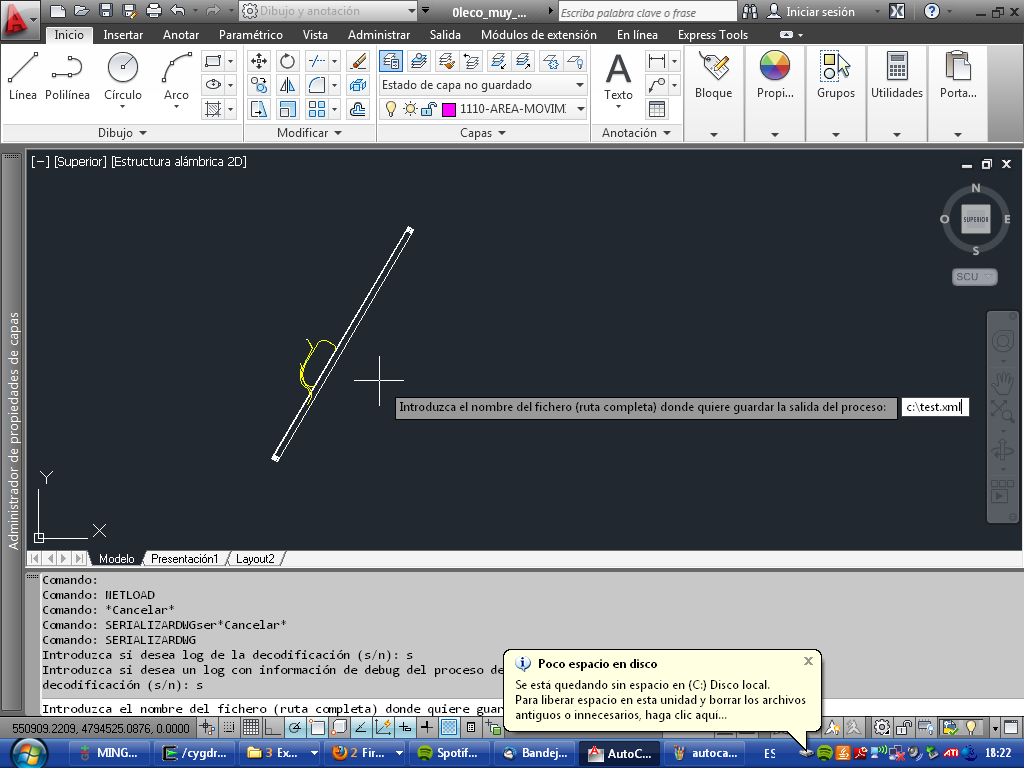
\includegraphics[width=\textwidth]{imgs/autocad8}
\caption{Usuario configurando la ruta donde se almacenará el fichero con la salida del proceso de extracción.}
\end{center}
\end{figure}

\begin{figure}[h]
\begin{center}
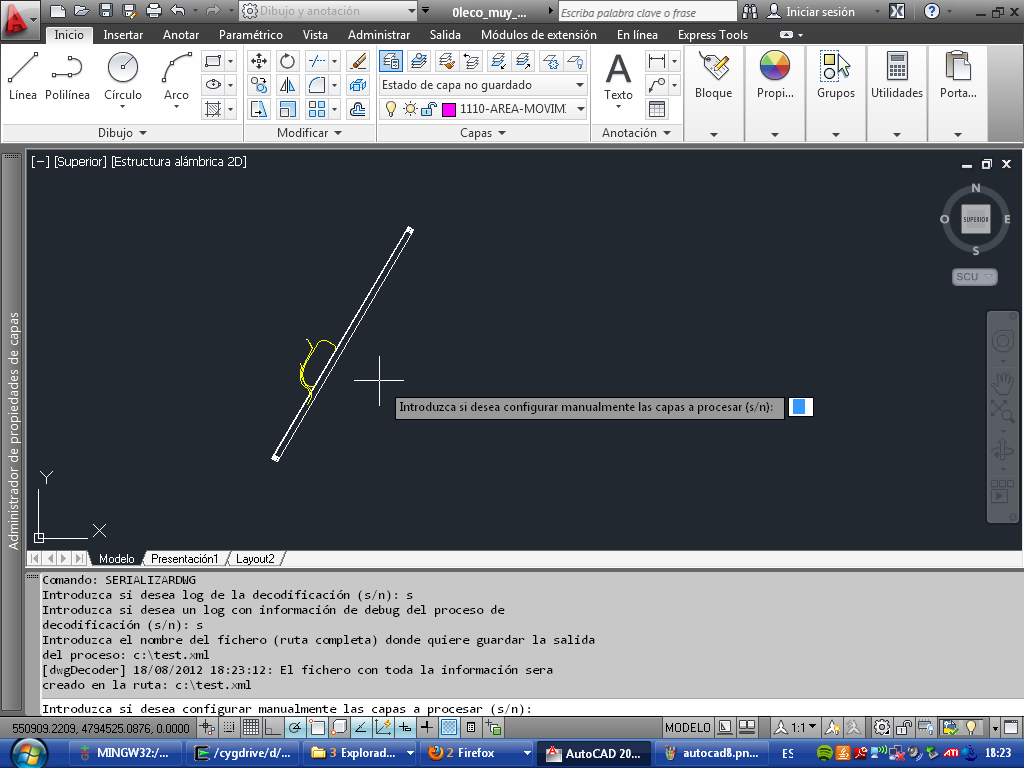
\includegraphics[width=\textwidth]{imgs/autocad9}
\caption{Usuario configurando si desea seleccionar las capas que deben ser procesadas.}
\end{center}
\end{figure}

\begin{figure}[h]
\begin{center}
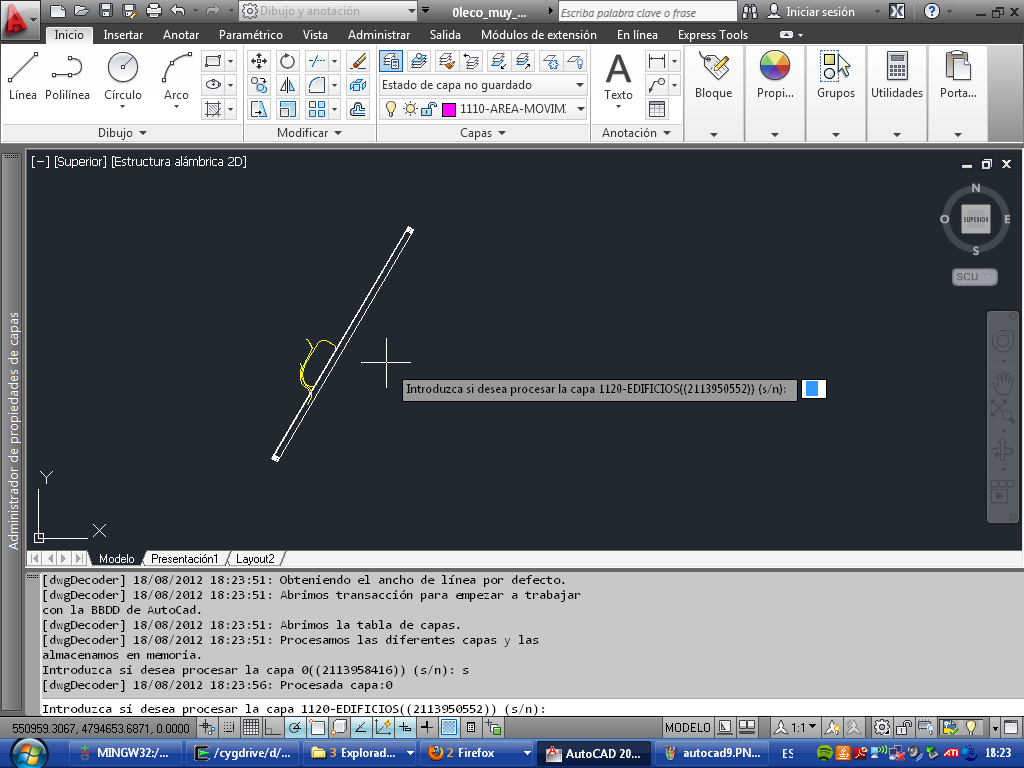
\includegraphics[width=\textwidth]{imgs/autocad10}
\caption{Usuario configurando si desea incluir una capa en el proceso.}
\end{center}
\end{figure}

\begin{figure}[h]
\begin{center}
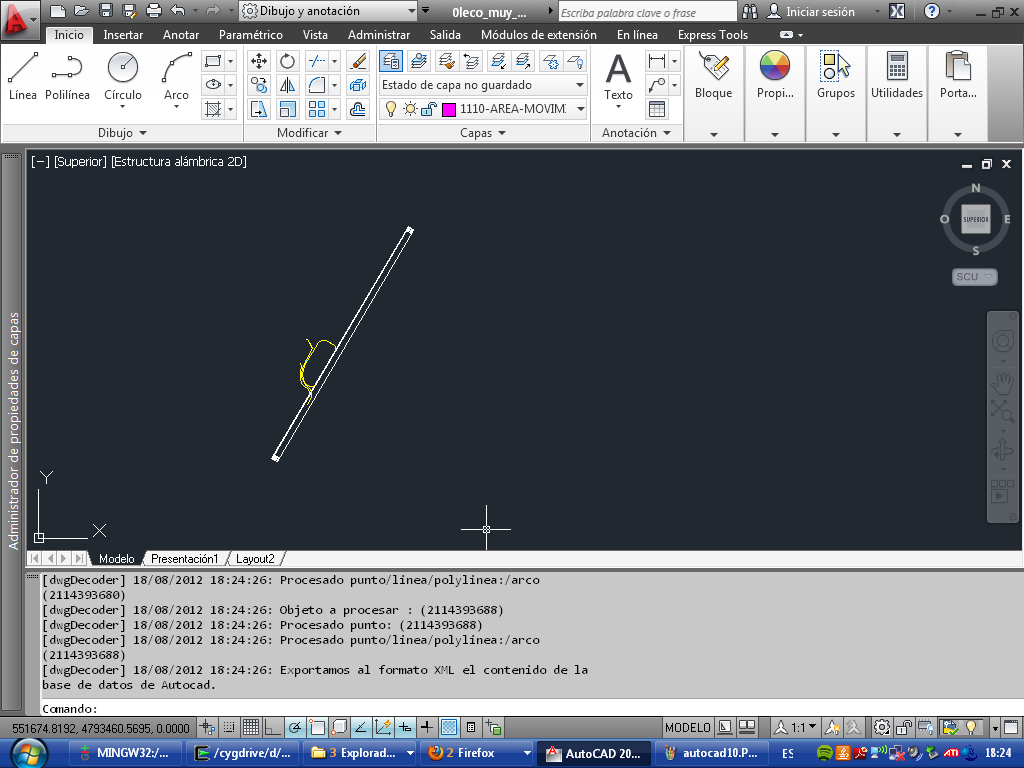
\includegraphics[width=\textwidth]{imgs/autocad11}
\caption{Aplicación AutoCad indicando que la exportación ha finalizado correctamente.}
\end{center}
\end{figure}



\section{Apendice 2. Ejemplo de salida del plugin SERIALIZARDWG.}

\lstinputlisting{xml/leco.xml}

\newpage \bibliography{references}
\newpage \listoffigures
%\listoftables

\end{document}
